%\section{OpenCV Port}
While the MATLAB Computer Vision system Toolbox is highly powerful and produced good results for our setup, there are drawbacks. Namely MATLAB is closed source software that requires payment to use. At the same time, MATLAB can be tedious to integrate with external applications and thus might not be ideal if camera calibration is only a part of a larger pipeline. OpenCV on the other hand is both widely used for a variety of image and computer visions applications, and is both open source and easy integrate. As noted earlier, OpenCV has implementations of camera calibration already and they are simple to use. Unfortunately they lack the user interface and built in outlier removal to make calibrating something like SuperView efficient. A similar implementation of the MATLAB outlier removal system was thus developed as an easy to use tool in OpenCV.

Because data visualization plays such a crucial role in identifying bad calibration input images, there needed to be a good way to generate interactive graphs of the OpenCV calibration results. This can be time consuming in C++, so alternatively python's Matplotlib library was used to recreate as similar output as possible to MATLAB's. OpenCV has both a C++ and a python library, but python was found to quite slow in calibrating large data sets. Due to this, a hybrid C++ and python application was created. The finalized control flow is as follows. 

\begin{enumerate}
	\item The C++ application reads in a set of input image pairs for calibration
	\item The calibration board corner points are detected and stored in an external file
	\item The first calibration run takes place and the reprojection error of every input image is stored in an external file along with the average reprojection error
	\item A python script reads the reprojection errors and plots them along with an average reprojection error line
	\item The user adjusts the average reprojection error line, selects outlier removal button, and the file of corner points is edited down to the new smaller set
	\item The C++ application reads in the corner points, avoiding time spent calculating the corner points again, and recalculates the reprojection errors with the new set
	\item The output is again used in the python script and the process is repeated
\end{enumerate}

Fig. \ref{fig:cvrepro} shows the plot generated by the OpenCV port, and the reprojection error for the image set of \ref{fig:results1}. After iterative outlier removals, the error is brought down from the original 2.83 to 1.02. This compares to MATLAB's error output of .51. Because MATLAB is a closed source application, the exact method for calibration can not be ported over directly. This means MATLAB's calibration probably involves a slightly refined calculation and optimization. OpenCV has trouble matching MATLAB's results and its speed, but compared, but this method still provides an open source alternative. These results match or are even better than hand picking input images and saves time eliminating bad options. 

\begin{figure}[th]
	\centering
	\fbox{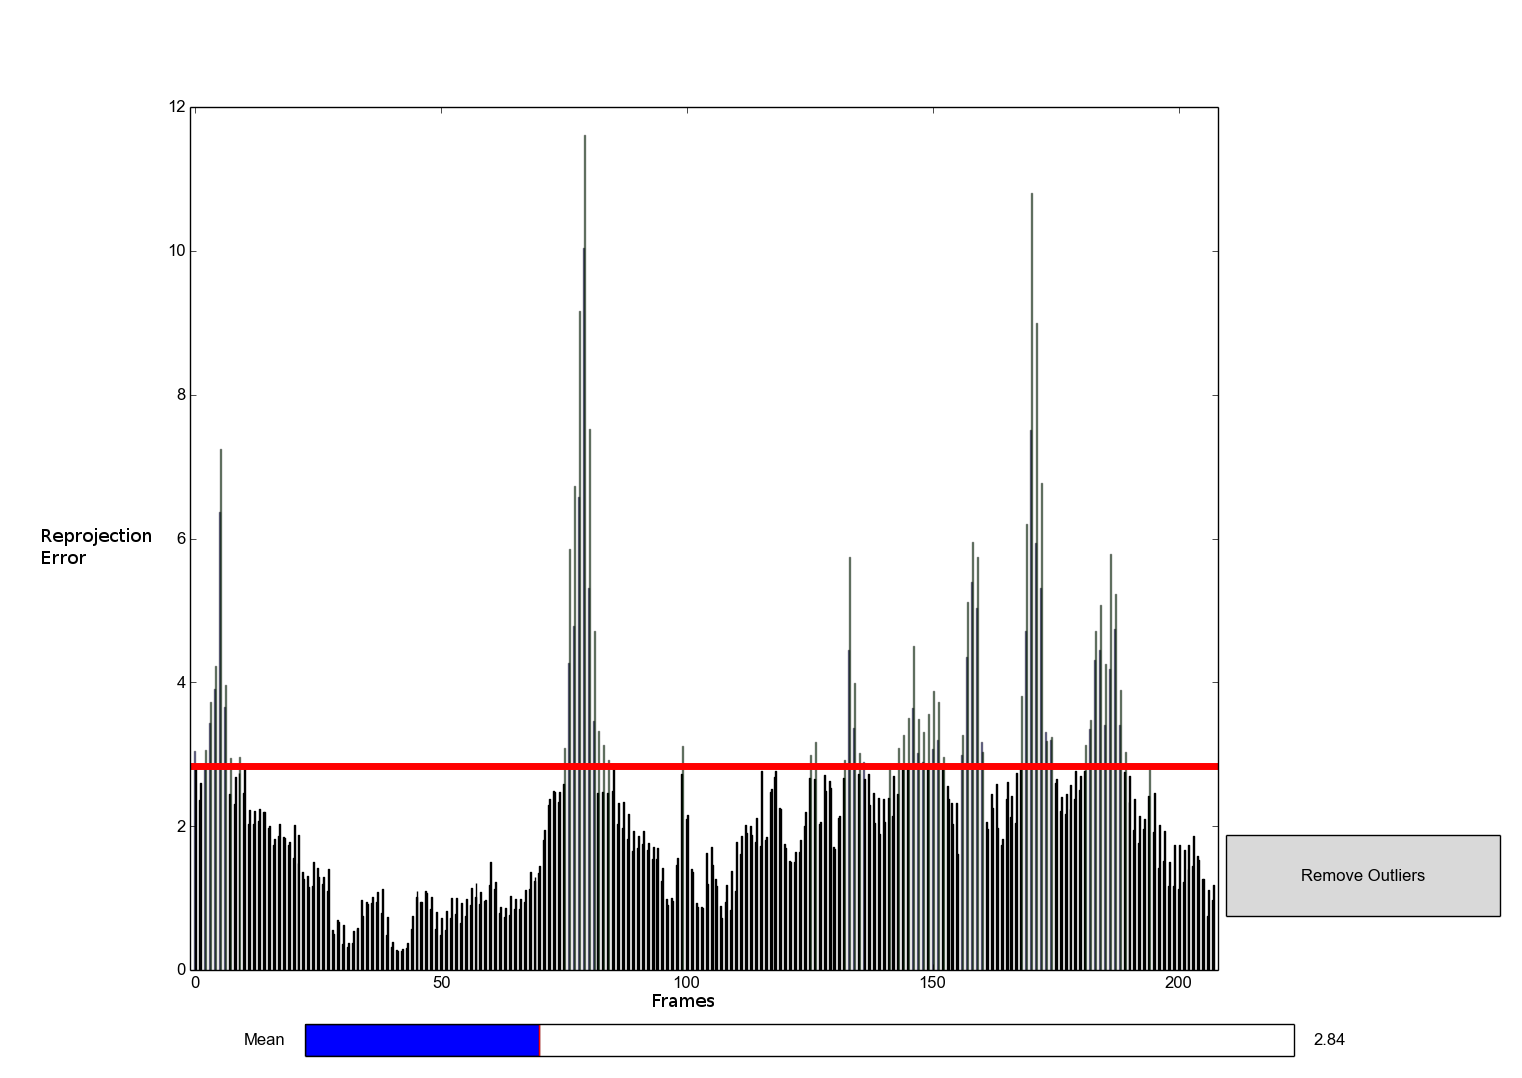
\includegraphics[width=0.95\textwidth]{./figures/allframes_axes_labels}}
	\caption{Initial reprojection errors plotted in python}
	\label{fig:cvrepro}
\end{figure}